\section{A \SemiEmpirical Theory of (Deep) Learning (\SETOL)}
\label{sxn:setol}
Based on prior empirical results, and the success of the \ALPHA and \ALPHAHAT metrics that are based on the \HTSR \Phenomenology, this leads to the deeper question: 
%
\begin{quote}
\emph{Why do the \ALPHA and \ALPHAHAT metrics work so well as NN model quality metrics for SOTA NN~models?}
\end{quote}
That is, why do NN models with heavier-tailed layer Empirical Spectral Distributions  (ESDs) tend to generalize better when compared to related models, and how can single-layer metrics predict model quality so well ?
Relatedly, can we derive these metrics from first principles?
(If so, then under what conditions do they hold, and under what conditions do they fail?)

\noindent
To answer these questions, we will derive a general expression for the \LayerQuality, $\Q$, of an NN.
Although many modern NNs have many layers, we adopt a single-layer viewpoint (like a matrix-generalized Student–Teacher) because in \StatisticalMechanicsOfGeneralization (\SMOG) theory~\cite{SST92,STS90} the multi-layer generalization can be factorized or approximated.
For this, we will obtain by simple averaging our model quality metrics, under effectively a single layer approximation, that correspond to \ALPHA and \ALPHAHAT.


In deriving these quantities, we will introduce to NN theory a new \SemiEmpirical approach that combines techniques from \STATMECH and \RMT in a novel way.must depend on the spectral density
The \LayerQuality $\Q$ will estimate the contribution that an individual NN layer makes to the overall quality of a trained NN model.
In deriving $\Q$, we have discovered a new \LayerQuality metric, called the \TRACELOG condition,
which indicates that the generalizing components of the layer must concentrate into a low-rank subspace which we term the \emph{\EffectiveCorrelationSpace}, or~\ECS. That is, the better this condition is met, the more the generalizing components concentrate in this \ECS, and this tendency provides a new layer quality metric, derived in a totally independent way from \ALPHA and \ALPHAHAT. We will provide strong empirical justification that both metrics are acceptable Quality metrics by showing that they converge as model quality increases.

%\red{[There are forward pointers to \ref{sxn:empirical}, but not to \ref{sxn:matgen}. \ref{sxn:matgen} fulfills the claims of derivation. I suggest to start a new paragraph here, and add one above that does a similar job relating results in Section \ref{sxn:matgen} to claims being made here. This is one of the most critical pages in the whole paper.]}\\
Importantly, we have conducted detailed experiments to show 
that the empirical estimates of the \SETOL \TRACELOG condition align remarkably well with predictions from the \HTSR
theory under \Ideal conditions (see Sections~\ref{sxn:empirical-test_acc}) and, then, 
that the key assumptions of our \SETOL theory are valid
(see Sections~\ref{sxn:empirical-effective_corr_space} and \ref{sxn:empirical-trace_log}).
In Section~\ref{sxn:empirical_comp_r_transforms}, we demonstrate how to apply theory directly using explicit calculations of the \RMT layer cumulants.
We next examine how the \HTSR predictions (i.e., the HT PL exponent $\alpha$) behave under non-\Ideal conditions (see Sections~\ref{sxn:empirical-correlation_trap} and \ref{sxn:hysteresis_effect}).
%
In the following, we will outline key conceptual aspects of \SETOL.
In Section~\ref{sxn:setol_overview}, we give an overview of \SETOL;
In Section~\ref{sxn:ideal_learning}, we describe the conditions of \Ideal learning under \SETOL and how they differ from those of \HTSR; and
In Section~\ref{sxn:HT_ESDs} we describe conditions that deviate from this.

\begin{figure}[htbp]                 % place here / top / bottom / page
  \centering
  % --- scale the entire picture to 75 % ---
  \scalebox{0.75}{% ---------- flowchart.tex ----------
\usetikzlibrary{arrows.meta, positioning, calc}

\tikzset{
  box/.style={
    draw, rectangle, rounded corners=3pt,
    minimum width=4.3cm, minimum height=1.3cm,
    align=center, font=\small
  },
  arrow/.style={-Stealth, very thick},
}

\begin{tikzpicture}[
  node distance = 2.5cm and 2.3cm,
  >=Stealth
]

% ========== ROW 1 ==========
\node[box] (smog)    {\underline{Classic SMOG}\\Student-Teacher Perceptron\\
but with  \\
\textbf{Fixed Teacher (input)}};
\node[box, right=of smog] (overlap)
      { \underline{ST Accuracy (Quality) $\Q^{ST}$} \\
    Thermal Average (AA, high-T) \\
        Overlap $R=\SVEC^{\top}\TVEC$ \\
      $\Q^{ST}=\THRMAVG{R}$ 
      };
\node[box, right=of overlap] (hciz)
      {\underline{Matrix Generalized Quality $\QT$}\\
      HCIZ Integral \\
$\OVERLAP:=\tfrac{1}{N}\SMAT^{\top}\TMAT$ \\
$\QT :=   \THRMAVGIZ{\Trace{\OVERLAP^{\top}\OVERLAP}}$  \
      };

% ========== ROW 2 ==========
\node[box, below=of smog] (rg)
      {
        \underline{Wilson Exact RG Condition (\ERG)}\\
      {Effective Correlation Space (\ECS)}\\[4pt]
      $\AMATN=\tfrac{1}{N}\SMAT\SMAT^{T}$, $\AECS=\mathbf{\hat{P}}^{ECS}\AMATN$ \\[4pt]
      $d\mu(\SMAT)\rightarrow  d\mu(\AMAT) \rightarrow d\mu(\AECS)$ \\[4pt]
      $\sum \ln \LambdaECS = 0 $  , $\LambdaECS \ge \LambdaECSmin $
      };

\node[box, below=of overlap] (tanaka)
      {\underline{Tanaka Result for HCIZ}\\
      \LargeN in $N$ limit \\[6pt]
      $\IZG = \tfrac{1}{N}\ln \int d\mu(\AECS)
      exp[n\beta N \Trace{\tfrac{1}{N}\TMAT^{\top}\AMATN\TMAT}]$\\[4pt] 
      $\QT := \tfrac{\partial }{\partial n}\tfrac{1}{\beta}\IZGINF$
      };

\node[box, below=of hciz] (cumul)
  {\underline{Integrated \RTransforms} \\[4pt]    
     $\QT = \sum_{\LambdaECS}\int_{\LambdaECS_{min}}^{\LambdaECS}R_{\AECS}(z)$ \\[4pt]  
     Student ESD $\AMAT$ $\sim$ Teacher ESD $\XMAT$ \\
   $R_{\AECS}(z) = R_{\XECS}(z)$
   };

% ========== ROW 3 ==========
\node[box, below=of rg] (rforms)
      {\underline{\RTransform choices}\\
      Bulk+Spikes (BS) \\
      Free Cauchy (FC)  \\ 
      Inverse MP (IMP) \\
      L\'evy Wigner (LW) \\
      $\cdots$
};

\node[box, right=of rforms] (alpha)
      {\underline{Derive \HTSR metrics}\\
      Extend \SETOL to non-Ideal cases \\\
      $\alpha$ and $\hat{\alpha}$};

\node[box, right=of alpha] (expv)
      {Experimental\\verification};

% ---------- horizontal arrows ----------
\draw[arrow] (smog)   -- (overlap);
\draw[arrow] (overlap) -- (hciz);

\draw[arrow] (rg)     -- (tanaka);
\draw[arrow] (tanaka) -- (cumul);

\draw[arrow] (rforms) -- (alpha);
\draw[arrow] (alpha)  -- (expv);

% ========== bridge 1 : HCIZ → RG  (↓ → ← → ↓) ==========
\coordinate (hcizDrop) at ($(hciz.south)+(0,-0.9)$);          % fall below Row-1
\coordinate (hcizLeft) at ($(hcizDrop -| rg.north)$);         % horizontal to col-1 x
\draw[arrow] (hciz.south) -- (hcizDrop)                       % vertical
             -- (hcizLeft)                                    % horizontal
             -- (rg.north);                                   % vertical down into RG

% ========== bridge 2 : Cumulants → R-forms (↓ → ← → ↓) ===
\coordinate (cumulDrop) at ($(cumul.south)+(0,-0.9)$);
\coordinate (cumulLeft) at ($(cumulDrop -| rforms.north)$);
\draw[arrow] (cumul.south) -- (cumulDrop)
             -- (cumulLeft)
             -- (rforms.north);

\end{tikzpicture}
}   % path to flowchart.tex (no “.tex” needed)

  \caption{Flowchart of the theoretical concepts used to construct SETOL.}
  \label{fig:cetl-flow}
\end{figure}
\subsection{\SETOL Overview}
\label{sxn:setol_overview}

\charles{Some old text here I need to clean up}

Our \SETOL formulates a parametric expression for the \LayerQuality $\Q$ using a matrix-generalization of the classic \StudentTeacher (ST)
model from the \SMOG theory of the 1990s~\cite{SST92,STS90}, evaluated using
recent advances in the evaluation of so-called HCIZ random matrix integrals~\cite{potters_bouchaud_2020,Tanaka2007, Tanaka2008},
such that the final expression for $\Q$ can be written in terms of empirically measured statistical properties of the layer ESD.
We summarize our basic approach here; see Section~\ref{sxn:matgen} for a detailed derivation, and see Section~\ref{sxn:empirical} for a detailed empirical analysis.

Following the \StudentTeacher (ST) model~\cite{SST92}, 
we first formulate the \GeneralizationError $(\AVGE^{ST}_{gen})$ of the linear \Perceptron (in the \emph{\AnnealedApproximation},
and in the \emph{\HighTemperature} limit; see Section ~\ref{sxn:SMOG_main}), and 
we then generalize this to the case of a NN $(\AVGE^{ST}_{gen}\rightarrow\AVGE^{NN}_{gen})$, so that we can analyze the \Quality of each layer.
For the \Perceptron, the \GeneralizationError is an Energy, given as $\AVGE^{ST}_{gen}:=\THRMAVG{1-R}$, where $R$ is the ST vector overlap,
and $\THRMAVG{\cdots}$ is a \emph{\ThermalAverage} (defined in Section~\ref{sxn:mathP}),
a Boltzmann-weighted average.
In this case, the model \Quality, $\Q^{ST}$ is exactly the AA, high-T \AverageGeneralizationAccuracy 
\michaeladdressed{still not sure we are using that term correctly, here and elsewhere}
$\Q^{ST}:=1-\AVGE^{ST}_{gen}=\THRMAVG{R}$.
For an MLP or general NN, each layer Energy is associated with a
\LayerQuality $\Q$, which we identify as the average contribution an
individual layer makes to the overall generalized accuracy,
(i.e $1-\AVGE^{NN}_{gen}$) for a multilayer perceptron (MLP).

For technical reasons (below), we will seek the
\emph{\LayerQuality (Squared)} $\QT$, which is defined as the \ThermalAverage
of the matrix-generalized overlap ($\Trace{\OVERLAP^{2}}$),
\begin{align}
  \label{eqn:QT}
  \QT :=   \THRMAVGIZ{\Trace{\OVERLAP^{2}}}
\end{align}
where $\OVERLAP^{2}$ can be thought of as a \Hamiltonian for the \QualitySquared  $(\HBARE=\OVERLAP^{\top}\OVERLAP)$.

In \EQN~\ref{eqn:QT}, the so-called \emph{\Teacher} ($T$) is the NN model under consideration,
%where $\mathbf{T}$ and $\mathbf{S}$  are the \Teacher and \Student layer weight matrices, resp,
and 
%$\mathbf{R}$ 
$\mathbf{R}:=\frac{1}{N}{\mathbf{S}^{\TR}\mathbf{T}}$
denotes the ST overlap operator 
between the \Teacher layer weight matrix $\TMAT$ and a similar \emph{\Student} ($S$) layer weight matrix $\SMAT$.
The notation $\THRMAVGIZ{\cdots}$ denotes a \ThermalAverage over
all \Student weight matrices $\mathbf{S}$ that resemble the \Teacher weight matrix $\mathbf{T}$.
By ``resemble'', the \SETOL approach assumes that 
%$\mathbf{S}$ lies in the same \HTSR Universality class as the $\mathbf{T}$, and, even more, that 
the ESD of $\mathbf{S}$ has the same \emph{limiting} form as $\mathbf{T}$, placing them in the same \HTSR Universality class.
This is made more precise below.

Let us now express the average matrix-matrix overlap $\mathbf{R}$ in squared form using:
\begin{align}
  \label{eqn:R2}
\Trace{\OVERLAP^{2}} &:=\OLAPSQD  \\ \nonumber
&=\frac{1}{N^{2}}\Trace{\mathbf{T}^{\TR}\mathbf{SS}^{\TR}\mathbf{T}}
=\frac{1}{N}\Trace{\mathbf{T}^{\TR}\mathbf{A}_2\mathbf{T}}
\end{align}
where $\AMAT_{2}$ is the $N\times N$ form of the \Student correlation matrix,
$\mathbf{A}_2:=\frac{1}{N}\mathbf{SS}^{\TR}$.
We will also define the $M\times M$ matrix, $\AMAT_{1}=\frac{1}{N}\mathbf{S}^{\TR}\mathbf{S}$,
used later.

\michaeladdressed{Clarify.}
%It is argued that the \Student and \Teacher weight matrices (i.e., $\TMAT, \SMAT$) have
%specific generalizing eigencomponents that, after training,
%concentrate in a low rank subspace, called the \emph{\EffectiveCorrelationSpace} (\ECS)
%(and that this space satisfies the \TRACELOG condition, described below).
%This is both consistent with the empirical observations and necessary to apply the HCIZ integral
%methods, both described below.
\michaeladdressed{MM TO DO: Dense.  Where is the best place for this par.}

As explained in Section~\ref{sxn:mathP}, this \QualitySquared is more readily obtained as 
the derivative of the \LayerQualitySquared \GeneratingFunction, $\IZG$, defined as
\begin{align}
  \label{eqn:IZG_QT}
  \QT := \dfrac{1}{\beta}\dfrac{\partial }{\partial N} \lim_{N\gg 1}\IZG
\end{align}
$\IZG$ is essentially ($\beta$ times) a \emph{\FreeEnergy} for the (approximate) \LayerQualitySquared.
(see Section~\ref{sxn:SMOG_main}, and the Appendix, Section~\ref{sxn:quality}).
For more details, see Section~\ref{sxn:matgen}, and the Appendix, Section~\ref{sxn:summary_sst92}).

We can write $\IZG$ as an HCIZ Integral, 
\begin{align}
  \label{eqn:QT_dS}
  \IZG  &=  \ln\int d\mu(\mathbf{S})\exp\left(N\beta\Trace{\mathbf{T}^{\TR}\mathbf{A}_2\mathbf{T}}\right),
\end{align}



The \SETOL approach then seeks to express $\IZG$ in~\EQN~\ref{eqn:QT_dS} as an HCIZ integral (and in the large-N limit)~\cite{potters_bouchaud_2020,Tanaka2007,Tanaka2008}.
We evaluate this at large-$N$, and write
\begin{equation}
  \IZGINF:=\lim_{N\gg 1}\IZG
\end{equation}
%%%must restrict the matrices to a lower rank subspace, called the~\ECS,
%%%i.e.,  $\mathbf{\tilde{A}}$. 
%%%We also must change the measure from an integral over \Student weight matrices
%%%to an integral over \Student Correlation matrices, i.e., 
%%%\begin{align}
%%%  \label{eqn:change_measure}
%%%  d\mu(\mathbf{S})\rightarrow d\mu(\mathbf{\tilde{A}}) ,
%%%\end{align}
%%%We can define a single measure for either form of \Student correlation matrix, restricted to the~\ECS,
%%%such that 
%%%$d\mu(\mathbf{\tilde{A}})=d\mu(\mathbf{\tilde{A}}_1)=d\mu(\mathbf{\tilde{A}}_2)$.
%%%This will be important as we need the form $\AMAT_1$ to derive the \TRACELOG condition, below, but
%%%we  formulate the  $\IZG$ using the form $\AMAT_2$.
%%%%Also, and importantly, the change in measure from $d\mu(\mathbf{S})$ to $d\mu(\mathbf{\tilder{A}})$
%is needed in order to apply the HCIZ  integral.
\michaeladdressed{I feel like expositionally it may be good to highlight this in the intro also and to have a bullet highlighting the rule from \HTSR for selecting the generalizing subspace; that will make it easier in the next subsection to highlight how the two connect.}
\charles{Lets discuss.  The intro has some of this. and a lot more}
With these definitions in place, moving forward, the following key assumptions, which can be tested empirically, must hold:
\begin{itemize}
  \item
  \textbf{The Effective Correlation Space (\ECS) Condition.}
  The generalizing components of the \Student (and \Teacher) layer weight matrices concentrate into a lower rank subspace---the~\ECS---spanned by the
  eigenvectors associated with the (heavy) tail of the layer ESD $\rho_{tail}(\lambda)$, such that the test error can 
  be reproduced with only these components. 
  \michael{MM TO DO: we need to define tail better somewhere, but see also my comment above about presenting the two generalizing subspaces better.}
  We write $\AECS$ to denote the projection of the correlation
  matrix $\AECS:=\mathbf{P}_{ecs}\AMAT$, onto this subspace, now with rank $\MECS\ll M$.
  This restricts the measure $d\mu(\AMAT)$ to the~\ECS, $(d\mu(\AMAT)\rightarrow d\mu(\AECS))$.
  This assumption will empirically examined using real-world \Teacher weight matrices $\TMAT=\WMAT$
  in Section~\ref{sxn:empirical-effective_corr_space}. 
%  Importantly, this lets interpret the \EQN~\ref{eqn:QT_HCIZ}  as acting only in this subspace.
  \item
  \textbf{The \TRACELOG Condition.}
  The \Student correlation matrix $\AECS_1$ (when properly normalized)
  satisfies the condition that $\Trace{\ln\AECS_1}=\ln\Det{\AECS_1}=0$,
  so that the change of measure $d\mu(\SMAT) \rightarrow d\mu(\AECS) $ is Volume Preserving.
  This condition is derived explicitly in terms of $\AECS_1$, and therefore will hold for $\AECS_2$
  (and the Teacher Correlation matrix, $\XECS=\frac{1}{N}\TMAT^{\TR}\TMAT$).
  Practically, this implies that the $\MECS$ eigenvalues $\LambdaECS$
  of the tail of the ESD must satisfy $\sum_{i=1}^{\MECS}\ln\LambdaECS_{i}\approx 0$.
  Experiments will test this assumption explicitly in Section~\ref{sxn:empirical-trace_log}.
\end{itemize}
Remarkably, both conditions hold best empirically when the \HTSR PL quality metric $\alpha\gtrsim 2$ is \Ideal. Motivated from these empirical observations, we have:
\begin{itemize}
  \item
  \textbf{$\IZGINF$ is expressed as an HCIZ integral, at large-$N$.}
  We have
  \begin{align}
  \label{eqn:IZGINF_HCIZ}
  \IZGINF = \lim_{N\gg 1}\ln\int d\mu(\AECS)\exp\left(\beta\Trace{\mathbf{T}^{\TR}\AECS_2\mathbf{T}}\right) %= \beta\sum_{i=1}^{\MECS}\GNECS
  \end{align}
  where  measure $d\mu(\AECS)$ lets us average over all \Student Correlation matrices $\AECS_{2}$ which
  lie in the~\ECS space and which ``resemble'' the \Teacher, 
  where by ``resemble'' we mean that they share the same form of the tail of
  their limiting ESDs,
  i.e., $\rho^{\infty}_{\AECS}(\lambda)\sim\rho^{\infty}_{\XECS}(\lambda)$.
  \item
  \textbf{The Layer Quality (Squared) $\QT$ is a~\GEN.}
  \michael{We need to figure out what to call that, I think norm isn't right, is it a generating function.}
  \charles{OK go ahead.}
  The final expression for $\QT$ can be written as the derivative of $\IZGINF$  as
  \begin{align}
    \label{eqn:QT_result}
    \QT = \dfrac{1}{\beta}\dfrac{\partial}{\partial N}\IZGINF = \sum_{i=1}^{\MECS}\GNI
  \end{align}
  where $\GNI$ is a \emph{\GEN}, and is  defined as the integrated \emph{\RTransform} $R(z)$ of the \Teacher
  layer ESD (where $z\in\mathbb{C}$), such that $\GN:= \int_{\LambdaECSmin}^{\lambda}R(z)dz$
  and $\LambdaECSmin$  encapsulates  the~\ECS (and selects the desired branch-cut of $R(z)$
  so that it is both single-valued and analytic).
\end{itemize}


\michael{MM TO DO: Somewhere we need to distinguish between \SemiEmpirical in general and our specific \SETOL approach.}
%\charles{TRY THIS: These two key, testable assumptions allow \SETOL to move beyond the \HTSR \Phenomenology to derive a more rigorous expression of model \GeneralizationError. It does so by leveraging spectral properties of weight matrices that permit deeper characterization of ways in which weight \emph{matrices} can be similar -- or \ATypical -- which is something parameter \emph{vectors} cannot.}
%\michael{No, I understand that.  What I am asking is: how do we want to describe the difference between \SemiEmpirical and \SETOL?  I think \SETOL is our particular model and setup; but \SemiEmpirical is a more general approach (meaning, in particular, it may not need a bolded name here).  }
%\charles{OK, well we have a section (140) where we discuss nuclear physics; what about there ?}

To apply the theory, one must choose an \RTransform $R(z)$ for	the \Teacher that models 
the tail of the ESD $\rho^{emp}_{T}(\lambda)$, and that can be
parameterized by some measurable property.
This may include the number of Spikes $\lambda^{spike}$, the fitted PL exponent $\alpha$,
the maximum eigenvalue $\lambda_{max}$, or even the entire tail $\rho^{tail}_{T}(\lambda)$.
This may be a formal expression, a computational procedure, or some combination.

To integrate $R(x)$, however, to have a physicaly meaningful result,
one must ensure that $R(z)$ is both
analytic and single-valued on domain of interest, namely, the \ECS (and therefore
the (PL) tail of the ESD),  $z \ge \LambdaECSmin$.
Because the ESD is frequently \HeavyTailed (HT), this
\RTransform $R(z)$ may have a branch-cut, and it is expected that this will occur
at $z\le \LambdaECSmin$, corresponding roughly at or before the start of the \ECS.
In a sense, selecting the branch-cut $R(z)$ forces one to define the \ECS.

To complete the theopry, we
will also show that the \HTSR PL \LayerQuality metrics \ALPHA $(\alpha)$  and \ALPHAHAT $(\ALPHAHATEQN)$
can be formally derived directly from the \SETOL \LayerQuality $\Q$ by selecting the appropriate
\RTransform $R(z)$. In Section~\ref{sxn:r_transforms} we provide several possible
model $R(z)$ and the resulting \LayerQuality $\Q$.
\michaeladdressed{Huh?}

\paragraph{Renormalization Group Effective Hamiltonian}
The formulation of SETOL closely parallels the construction of an \EffectiveHamiltonian~$\HEFF$
via the \WilsonExactRenormalizationGroup~(RG) approach. Consider a \emph{\Bare} Hamiltonian $\HBARE$ for the \LayerQualitySquared,
defined as $\HBARE:= \mathbf{R}^{\TR}\mathbf{R}$.
We can express Eqn.\ref{eqn:QT_dS} in terms of this \Bare Hamiltonian $\HBARE$,
and rewrite Eqn.\ref{eqn:IZGINF_HCIZ} in terms of an \emph{\Renormalized} \EffectiveHamiltonian~$\HEFF$
that spans the \EffectiveCorrelationSpace~(\ECS). Formally, we have:
\begin{align}
\label{eqn:RG}
\ln \int d\mu(\SMAT)e^{N\beta \operatorname{Tr}[\HBARE]} \;\xrightarrow{RG}\; \lim_{N\gg 1}\ln \int d\mu(\AECS)e^{N\beta \operatorname{Tr}[\HEFF]} 
\end{align}
where the RG transformation is defined by the \ScaleInvariant \TRACELOG condition,
applied at large-$N$,
and where $\HEFF$ is defined implicitly through result for $\QT$ (Eqn.~\ref{eqn:QT_result}).
The result is, formally, a sum of the integrated \RTransforms $\GNI$.
In a sense, this result resembles (a non-perturbative form of) the Linked Cluster Theorem
in that the log \PartitionFunction is expressed as a sum of integrated matrix-generalized cumulants and/or self-energy.  And in analogy with \SemiEmpirical theories of Quantum Chemistry, the \HTSR \ALPHA $(\alpha)$ and \ALPHAHAT $\ALPHAHATEQN)$ enter as renormalized empirical parameters.
Most importantly, the \ScaleInvariant \TRACELOG condition can be verified empirically (See Section~\ref{sxn:empirical}.  
Importantly, in analogy with the Wilson RG theory, 
the \HTSR $\alpha=2$ resembles in spirit
an RG \emph{Universal Critical Exponent} at a phase boundary being between the \HeavyTailed 
(HT) and the \VeryHeavyTailed (VHT) phase of learning of the \HTSR theory.
This observation strengthens our argument that the \HTSR HT and VHT phases
are analogous to the generalizing and overfit phases, resp.,
of the classical \SMOG theories of NN learning.



\subsection{Comparing SETOL with HTSR: Conditions for Ideal Learning}
\label{sxn:ideal_learning}

%Although \SETOL is a \SemiEmpirical theory based on \STATMECH applied in a novel way to the ST model, 

The \SETOL approach establishes a starting point for developing a first-principles theory for modern NNs. %understanding of generalization, 
Among other things, by connecting with the \HTSR \Phenomenology, it lets us identify conditions for an \Ideal state of learning for an individual NN layer, under the Single Layer Approximation.
By \Ideal, we mean that the layer is being used most effectively i.e., in some sense it is at its optimal data load, and thus it is conjectured to result in the best model quality.

\textbf{The \Ideal State of Learning} is conjectured to be characterized by the following three conditions:
\begin{enumerate} 
\item \label{itm:ideal_1}
  the tail of ESD, $\rho^{emp}_{tail}(\lambda)$, can be well fit to a PL of $\alpha\approx 2$: $\rho^{emp}_{tail}(\lambda)\sim\lambda^{-2}$;
\item \label{itm:ideal_2}
  the eigenvalues in the tail, $\lambda_{i}$, satisfy the \TRACELOG~condition: $\sum_{i}\ln\lambda_{i}=0$; and
\item \label{itm:ideal_3}
  the generalizing components of the layer concentrate in the singular vectors associated with the tail of the ESD, 
         (\EffectiveCorrelationSpace).
  \michaeladdressed{@charles: do we have a way to test this third one?}
  \charles{Seriously ?!}
\end{enumerate}
In Section~\ref{sxn:empirical}, we will test and justify this conjecture.


%Wee offer the following conjecture:
%\begin{quote}
%The HT Universality classes used in the \HTSR \Phenomenology can be used by the \SETOL approach to characterize the state of convergence of a layer in a trained NN.
%\end{quote}

%The \TRACELOG states that eigenvalues in the tail of the ESD, call them $\rho^{emp}_{tail}(\lambda)$, satisfy the following condition: 
%$\log\prod\lambda_{i}=\sum\ln\lambda_{i}=0$ for $\lambda_{i}\ge\lambda_{max}$.
%This condition is completely independent of \HTSR Theory, and it simply requires that the basic setup and premises of our \SemiEmpirical approach holds.
%When combined with empirical results below (see \michael{XXX-XXX}), we can now state the following.

These claims are fundamentally about NN learning itself. 
They are motivated by our formulation of the \SETOL approach in our search for a practical predictive theory behind the HTSR \Phenomenology.
When $(\ref{itm:ideal_1})$ and $(\ref{itm:ideal_2})$ conditions hold for any layer, we conjecture that $(3)$ holds as well.
Moreover, when $(\ref{itm:ideal_1}-\ref{itm:ideal_3})$ hold for all layers, we conjecture the
NN has the lowest \GeneralizationError (and highest \ModelQuality) possible for given model architecture and dataset.
\michaeladdressed{@charles: Does \GeneralizationError mean ``modely quality'' or ``generalization error'' there?}

\michael{This par should maybe be above.}
Previous results have shown that the \HTSR quality metrics (\ALPHA,  \ALPHAHAT, etc.)  correlate very well with reported test accuracies,
as well as model quality on epoch-by-epoch basis.
\michael{Refs. And clarify.}
These results hold because, as indicated by the \HTSR theory, the PL exponent $\alpha$ characterizes both the quality of the layer and provides an after-the-fact measure of the amount of regularization.%
\footnote{By ``after-the-fact'', we mean that it provides a measure of the regularization in a layer, along the lines of the self-regularization interpretation of \HTSR Theory~\cite{MM18_TR_JMLRversion}. However, we do \emph{not} recommend that it be used as an explicit regularization parameter. Informally, this is since the ``easiest way to obtain HT ESDs is to make weight matrices HT element-wise; but this is \emph{not} what is observed in practice, and thus this is precisely \emph{not} what \HTSR Theory and our new \SETOL approach are designed to model.}
However, the \HTSR approach says nothing about the \SETOL \TRACELOG condition; and neither does the \SETOL approach require a minimum of $\alpha=2$ to obtain the best model quality, as observed by the \HTSR \Phenomenology.
Remarkably, we can show that $(1)$ and $(2)$ do hold \emph{simultaneously}, both in carefully designed experiments on a small model,
as well as for many pre-trained, high quality open-source models. 

%And generally speaking, smaller $\ALPHA$ corresponds to better model quality, and with the layer averaged $\langle\alpha\rangle\in[2,4]$ for the better performing models. 
%\michael{Redundant.}

%MIKE \michael{Can or should we connect our quality metric to a capacity metric from SLT?
%MIKE This \ProductNorm resembles a Capacity measure for NNs from traditional ML theory, where
%MIKE $\Vert\mathbf{W}\Vert$ may be, say, Frobenius Norm, the Spectral Norm, or even their ratio, the Stable Rank.
%MIKE Traditional theory, however, usually considers metrics that only measure the \Scale of the layers.%}

\michael{Where to have this par?}
\michael{The following is an important point.  Probably it should be in the intro and only reminded of here.}
\HTSR theory, however, has been developed as a \Phenomenology describing the best trained, most accurate open-source models available.
As such, it may be biased towards such models, and it may not describe less optimal learning scenarios.
\michael{Weave that in in some way; that is probably better in the intro.}
The keys goals of this work are to derive independent conditions, both theoretical and experimental, that can
identify the conditions for \IdealLearning, and to stress-test these conditions in carefully designed,
reproducible experiments.
\michaeladdressed{How does that sentence relate to \SETOL, since one could have a \SETOL for lower-quality models.}
\charles{it is doubtful that the \TRACELOG condition would hold for a low-quality model. }


\subsection{Detecting Non-Ideal Learning Conditions}
\label{sxn:HT_ESDs}

%We would like to address the basic question:
%\begin{quote}
%What is the origin of the HT structure in the tail of the ESD?
%\end{quote}

The \HTSR \Phenomenology posits that SGD training reduces the \emph{\TrainingError} by accumulating correlations into the large eigenvalues
in NN layer weight matrices  $\mathbf{W}$ such that they \emph{self-organize} into a HT with a PL signature,
and that this successful self-organization leads to good model quality.
Conversely, it also posits that when training has gone awry in some way, the resulting ESD, $\rho^{emp}(\lambda)$, will
be deformed in some way.   
In many practical situations, there can be other, 
competing factors that give rise to large eigenvalues $(\lambda>\lambda^{+})$
that do not contribute to the generalization capacity of the model, and, consequently, 
can affect the \Scale (i.e., the largest eigenvalue(s) $\lambda_{max}$) 
and \Shape (i.e., the PL exponent $\alpha$, or goodness of fit $D_{KS}$) of the layer ESDs.
These large $\lambda$ could be \DragonKings, \emph{\CorrelationTraps}, or some other anomaly.

To apply the HTSR \Phenomenology most effectively, one must be able to identify various spurious factors and
distinguish real correlations from any other large eigenvalues, including the effects of both
extreme eigenvalues $\lambda$, individual matrix elements $W_{i,j}$, and rank-$1$ perturbations in $\WMAT$.
In one case the ESD is HT primarily due to correlations that help the model generalize, whereas
in another when the ESD may be more HT than expected due to suboptimal training, mis-labeled data, etc.
In extreme cases, spurious eigenvalues can push the weight matrix
into the \VeryHeavyTailed \Universality class (i.e., $\alpha<2$. See Table~\ref{tab:Uclass}, Section~\ref{sxn:htsr}), or
disrupt the formation of a HT, resulting in a poor PL fit, undermining the core proposition of the  \HTSR approach.

When training a model with SGD, one may only achieve  a sub-optimal result
when using overly large learning rates / small batch sizes, (see Section~\ref{sxn:empirical}),
from poor hyper-parameter settings,
or simply because direct regularization fails. In such cases, the \HTSR approach allows one to detect
potential problems by looking for large eigenvalues~\emph{not} resulting from correlations~\cite{GSZ20_TR}.

Importantly, in the context of the \SETOL theory, we can now identify such empirical anomalies
due to \ATypical layer weight matrices $\mathbf{W}$, a key factor when models break down.
The \SETOL approach formalizes the empirical \HTSR \Phenomenology,
%(and as a single layer theory),
but, in doing so, assumes that the
underlying layer effective correlation matrix $\XECS$, is~\Typical, meaning that it can describe out-of-sample / test data.
%\st{(This is because \SETOL is formulated in the annealed approximation; see Section XXX)}
Conversely, if the underlying weight matrix $\mathbf{W}$ is~\ATypical, then it is in some sense
overfit to the  training data and can not fully represent out-of-sample / test data.
Consequently, when $\mathbf{W}$ is \ATypical,  we argue that we can observe this, either in the ESD $\rho^{emp}(\lambda)$ directly
(i.e., when $\alpha< 2$),
and/or having $1$ or more unusually large matrix elements $W_{ij}$.

We conjecture such sub-optimal results, and particularly those occurring from overfitting, actually
arise when the underlying layer weight matrix $\mathbf{W}$ is \ATypical in some way,
in analogy to the results from the classic \SMOG theory (see Section~\ref{sxn:trad_smog}),
and, importantly, that we can use the \SETOL approach to detect when $\mathbf{W}$ is~\ATypical
and therefore a layer is overfit in some way.

%That is, if $\mathbf{W}$ is \ATypical will arise as \Shape and/or \Scale anomalies.
%Very Heavy Tailed ESDs may arise from a variety of phenomena, such as using too-small batch sizes, too-large learning rates, using ``bad data, etc.---all of which result in sub-optimal %t5raining.

Here, we identify two specific cases of \ATypical weight matrices---\CorrelationTraps and \emph{\OverRegularization}.% 
\footnote{Later, in Section~\ref{sxn:empirical}, we will show that we can systematically induce both phenomena and observe their effects on the \HTSR HT PL metric $\alpha$ and the \SETOL \TRACELOG condition.}
\begin{enumerate}[label=3.3.\arabic*]
  \item 
  \textbf{\CorrelationTraps.} 
  $\mathbf{W}$ is \ATypical in that $\mathbf{W}$
 exhibits an anomalously large mean $(\bar{\WMAT})$.  
  \michaeladdressed{Here ane below, what does mean? Mean of what?}
  We can observe these by randomizing the layer weight matrix, $\mathbf{W}\rightarrow\mathbf{W}^{rand}$, and then looking
  for eigenvalues that extend significantly beyond the MP edge of the random bulk (i.e., Spikes).  We call such random spikes
  \emph{\CorrelationTraps},  denoted as $\lambda_{trap}$, because they appear, in some extreme cases, to be associated with distorted ESDs
  and, importantly, lower test accuracies.  Examples of \CorrelationTraps are shown in Section~\ref{sxn:empirical-correlation_trap}.
  \item 
  \textbf{\OverRegularization.} 
  $\mathbf{W}$ is \ATypical in that $\mathbf{W}$ exhibits an anomalously large variance $(\sigma^2(\WMAT))$. 
  We can observe this when the layer  $\alpha < 2$.  Also, since \ALPHA a measure of implicit regularization, we say the layer with $\alpha<2$ is \emph{Over-Regularized}.
  In particular, when one layer is undertrained, having $\alpha>6$, it appears that other layers may become overtrained to compensate, and this can be seen with having $\alpha < 2$.
  These effects are studied in Section~\ref{sxn:empirical}.
  Additionally, we also observe that when evaluating the \SETOL \TRACELOG condition, when $\alpha < 2$, then $\Delta \lambda_{min}< 0$ (see Section~\ref{sxn:empirical-trace_log}).

\end{enumerate}
\michael{These are more saying what we see than seems right.}
\charles{WHY ?}

%These is only a few of the kinds of factors that can cause an ESD to have spurious heavy tails.


% MM: The following are three subsubsections, maybe incorporate them into this file.
\subsubsection{Correlation Traps}
%\paragraph{Correlation Traps.}
\label{sxn:Traps}

The first way we identify $\mathbf{W}$ as \ATypical is when it has an anomalously large mean $(\bar{\WMAT})$;
detecting this in general, however, requires more than just examining which elements $W_{i,j}$ are
anomalously large (because they may be a rank-1 perturbation consisting of more than one element).  Here, we can apply elementary RMT, as in the \HTSR approach.

The \HTSR \Phenomenology states that NNs generalize better when their layers ESDs are more HT---precisely because the 
tail eigenvalues arise from correlations in the weight matrices.
So one way is to identify \emph{atypicality} is to look for  large eigenvalues that
do not arise from correlations in $\mathbf{X}$,
but, rather, from one or a few spuriously large matrix elements $W_{i,j}$ and/or rank-1 perturbations in $\mathbf{W}$.
We call these eigenvalues  \CorrelationTraps, denoted by $\lambda_{trap}$
(i.e., see Section~\ref{sxn:empirical-correlation_trap}).

Indeed, if we randomize $\mathbf{W}$ element-wise, i.e $\mathbf{W}\rightarrow\mathbf{W}^{rand}$, we
expect the $W^{rand}_{i,j}$ matrix elements to be i.i.d and with a small mean
(unless something odd happens during SGD training).
Likewise, we expect the singular values of $\WMAT^{rand}$ to follow the MP distribution, to within
finite-size / TW fluctuations.
If we observe an eigenvalue $\lambda_{trap}$ extending beyond the MP bulk region, $\lambda_{trap}>\lambda^{+}_{bulk}$,
then the mean $W_{i,j}$ matrix element will also be anomalously large,
and we can identify $\mathbf{W}$ as \ATypical.
We must be careful, however, as we do not fully understand the origin of these atypicalities
and do not claim that every one is associated with suboptimal generalization.

By a \emph{\CorrelationTrap}, we mean that some anomaly in the training of $\mathbf{W}$ resulted
in one or more spuriously large eigenvalues $\lambda_{trap}$ in $W^{rand}$,
and that  whatever caused them also may, in some pronounced cases, tend
to ``trap the correlations in $\mathbf{X}$ itself,
preventing them from coalescing into a well defined PL Heavy Tail,
or otherwise distorting the ESD.
Whether they are a signature of training gone wrong, or whether they distort the dynamics of the tail correlations 
simply by being there, \CorrelationTraps can be expected to alter the shape of the ESD,
reducing the quality of the PL fits, and sometimes producing spurious $\alpha$ values.

Why would such anomalies occur in a NN?
It is conceivable that SGD will, when it fails to find usable correlations, instead
produce spurious
correlations in the form of large elements and/or rank-1 perturbations.
Also, the matrix itself may simply undergo an innocuous  mean-shift because the
mean is not explicitly controlled during training. Here,  mean-recentering may be beneficial.
\footnote{Similarly, when training NNs, frequently the weight matrices~\cite{baskin2021} or activations~\cite{choi2018_TR}
may need to be clipped during training to ensure good results.}

We will see, below in Section~\ref{sxn:empirical}, that we can induce a \CorrelationTrap both by shrinking the batch 
size, or, equivalently, increasing the learning rate, and that this is associated with degraded model performance
and small $\alpha$.
We seek to identify specific ways of identifying such traps because we 
reason that the presence of foreign large eigenvalues may disrupt the self-organization of correlations – or that failed learning may produce them as a by-product.

\paragraph{Detecting Correlation Traps with \RMT.}

RMT suggests that when a matrix $\mathbf{W}$ has unusually large elements $W_{ij}$, then the ESD will have one or more large eigenvalues $\lambda_{trap}$ lying outside the bulk edge $\lambda^{+}_{bulk}$ of the ESD, as predicted by MP theory. 
One can detect these so-called \CorrelationTraps in a weight matrix $\mathbf{W}$ by performing the following:
\begin{enumerate}
\item randomize $\mathbf{W}$ element-wise to obtain $\mathbf{W}^{rand}$;
\item compute the ESD for $\mathbf{W}^{rand}$; and
\item look for large eigenvalues $\lambda_{trap}\gg\lambda^{+}_{bulk}$.
\end{enumerate}
\WW~looks for \CorrelationTraps ($\lambda_{trap}$) in the ESD of the randomized $\mathbf{W}^{rand}$, that are larger than 
$ \lambda_{trap}>\lambda_{bulk}^{+}+\Delta_{TW} , $ 
where 
$\lambda^{+}_{bulk}$ is the MP bulk edge $\Delta_{TW}$ are the associated finite-size Tracy Widom (TW) fluctuations. 
This procedure detects \emph{any} anomaly in the matrix weights that produce spuriously large eigenvalues. 
It is implemented in \WW (using the randomize option), which was used to generate the plots in Figure~\ref{fig:scale-shape}.

\begin{figure}[ht]
    \centering
    \subfigure[Well-formed ESD]{ 
      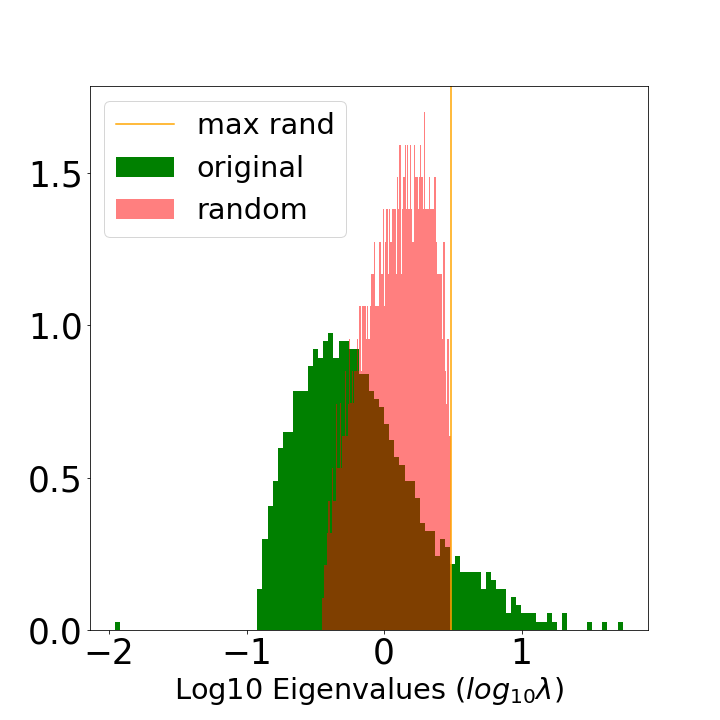
\includegraphics[width=7cm]{./img/shape-scale-a.png}
      \label{fig:scale-shape-a}
    }                               
    \subfigure[ESD with \CorrelationTrap]{                   
      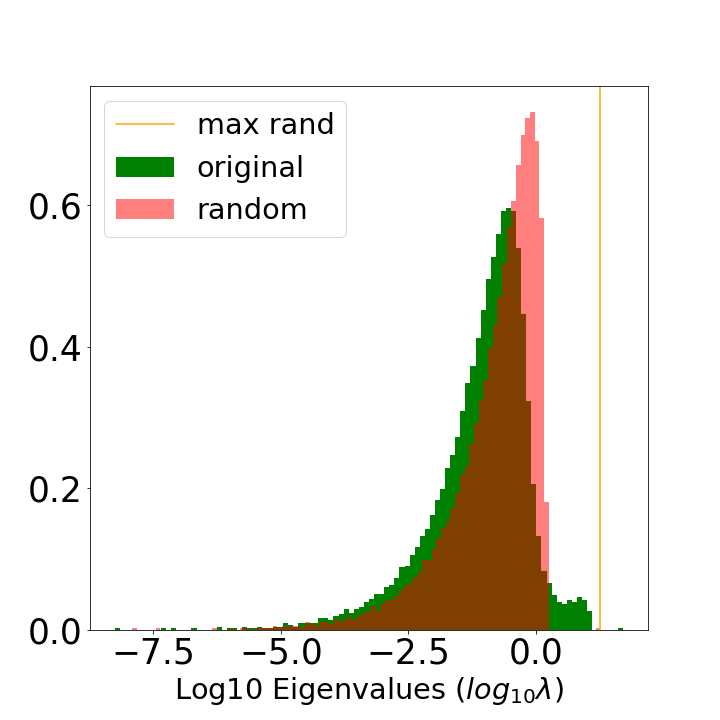
\includegraphics[width=7cm]{./img/shape-scale-b.png}
      \label{fig:scale-shape-b}                           
    }                                                                                                                            
    \caption{Comparison of a well-formed, Heavy-Tailed ESD (a) to one with a Correlation Trap (b), in the VGG16 model (FC2 layer)}
  \label{fig:scale-shape}                                                                                                      
\end{figure}

See Figure~\ref{fig:scale-shape-a}, which displays the (log)-ESD of a \Typical SOTA NN layer $\mathbf{X}$ (green), i.e., on a log-linear scale, along with the (log)-ESD of that layer after randomizing it element-wise (red).
The two ESDs differ substantially:
the ESD of the original weight matrix  $\mathbf{W}$ (green) is very HT, whereas 
the ESD of the randomized weight matrix  $\mathbf{W}^{rand}$ (red) is an MP (and as predicted by the MP \RMT).
The orange line corresponds to the maximum eigenvalue of the randomized ESD.
Note that it is at the MP bulk edge of the red plot, indicating that this ESD is not affected by unusually large elements or other weight anomalies.
Here, we say that the ESD of $\mathbf{X}$ is HT, and that $\mathbf{W}$ is not HT element-wise.
\HTSR says this layer is well trained.

Contrast this with Figure~\ref{fig:scale-shape-b}, which displays the (log)-ESD of a NN layer with a \CorrelationTrap.
The ESD of $\mathbf{X}$ (green) is weakly HT, but it looks nothing like the ESD in Figure~\ref{fig:scale-shape-a}.
In fact, it looks very much like the ESD of the randomized weight matrix  $\mathbf{W}^{rand}$ (red), except for a small shelf on the right. 
The orange line again corresponds to the maximum eigenvalue of the randomized ESD, and this is just past this shelf.
Relative to the randomized ESD, this line depicts (an) unusually large element(s)---or, equivalently, a rank-1 perturbation of $\mathbf{W}^{rand}$.
By a \CorrelationTrap, we mean that some anomaly in the elements of $\mathbf{W}$ tends to ``trap'' the ESD of $\mathbf{X}$, concentrating the correlations in $\mathbf{X}$ into the small shelf of density around the orange line. 
\HTSR says this layer is not well-trained because it does not have a good PL fit.

%We will see, below in Section~\ref{sxn:empirical}, that we can induce a \CorrelationTrap by shrinking the batch size, and that this is associated with a degradation in model performance (%as well as spuriously low PL exponent $\alpha$). 


%\paragraph{Correcting for \SCALE Anomalies with \ALPHAHAT}
%\subsubsection{Correcting for Scale Anomalies with \ALPHAHAT}

%\nred{repetitive ?}
%  \CorrelationTraps are a kind of \SCALE anamoly;by this we mean when the layer weight matrix $\mathbf{W}$
%  and/or the randomized  $\mathbf{W}^{rand}$ has one or more unusually large eigenvalues $\lambda$.
%  In the case of a scale anamoly, the simple PL \ALPHA metric may not correlate well with the test accuracy or other measures
%  of model quality because such scale anomalies may make it difficult to get a good PL fit of $\alpha$.
%  In some very hard cases, the layer ESD $\rho_{emp}(\lambda)$ may be significantly deformed from a well
%  behaved PL or TPL distribution (as in Fig.~\ref{fig:scale-shape-b}.  In these cases, the \ALPHAHAT
%  metric can frequently compensate.  This is seen in Section~\ref{sxn:empirical} \nred{see github issue 46}

 





\subsubsection{Over-Regularization}
\label{sxn:underfitting}

%\michael{Is the idea that this section parallels Section~\ref{sxn:Traps}, in that both describe non-\Ideal learning?  If so, we need to refine.  Are we saying that the primarily way $\alpha<2$ is when one layer is compensating for another.  }

The second way we identify $\mathbf{W}$ as \ATypical is when it has an anomalously large variance $(\sigma^2(\WMAT))$.
\michaeladdressed{Variance of what.}

The \SETOL theory -- a single-layer theory of learning -- casts the training 
of a NN layer in terms of how the correlations concentrate into the layer  \EffectiveCorrelationSpace (\ECS),
and becomes exact when the \TRACELOG condition is satisfied.
Analogously, the \HTSR theory -- a single layer \Phenomenology of learning -- casts training
of an N layer by fitting its ESD to a PL, and noting that the PL exponent $\alpha$ measures
the amount of implicit regularization in the layer.
Comparing the two approaches, we see that smaller $\alpha$ corresponds to the correlations
concentrating into a low-rank~\ECS.  In general, and likewise, the more the weight matrix
correlations concentrate  into a low-rank~\ECS, the better the layer has been regularized.
A natural question arises then, namely, can a layer be \emph{\OverRegularized} and
can we detect this?
and in large,
Empirically, we do indeed observe that over the course of training, $\alpha$ decreases, (See Figure~\ref{fig:mlp3-FC1-alpha-overloaded} 
(a), Section~\ref{sxn:hysteresis_effect},) and that the models predictions are concentrated into the~\ECS, 
(See Section~\ref{sxn:empirical-effective_corr_space}). Thus, we also interpret $\alpha$ and~\ECS concentration to be 
measures of learning itself, meaning that NNs are self-regularizing~\cite{MM18_TR_JMLRversion}.

Importantly, however, the \HTSR \Phenomenology indicates that \ALPHA usually lies in the Fat-Tailed Universality class,
such that $\alpha\in [2,6]$.  When $\alpha <2$, the ESD is Very Heavy Tailed (VHT), and, also,
this indicates that $\mathbf{W}$ has an anomalously large variance.  That is,  $\mathbf{W}$ is  \ATypical.
Occasionally, but very infrequently, we do observe $\alpha<2$, and in large, production quality models
(like Llama).
Interestingly, we also observe that, frequently, when the \HTSR $\alpha<2$, the \SETOL \TRACELOG
condition holds fairly well.  This is further explored in Section~\ref{sxn:empirical}

We have applied the \WW tool to have examined dozens
of modern, very large NNs; of particular interest are the so-called Large Language Models
(LLMs) that have revolutionized the field of AI.  To that end, in Figure.~\ref{fig:falcon_vs_llama},
we present the \WW layer \ALPHA metrics for the Falcon-40b and the Llama-65b LLMs.
\footnote{Similar results are found for the larger, more modern Llama models,
and can be found on the ~\WW website\cite{WW}}

\begin{figure}[ht!]
    \centering
    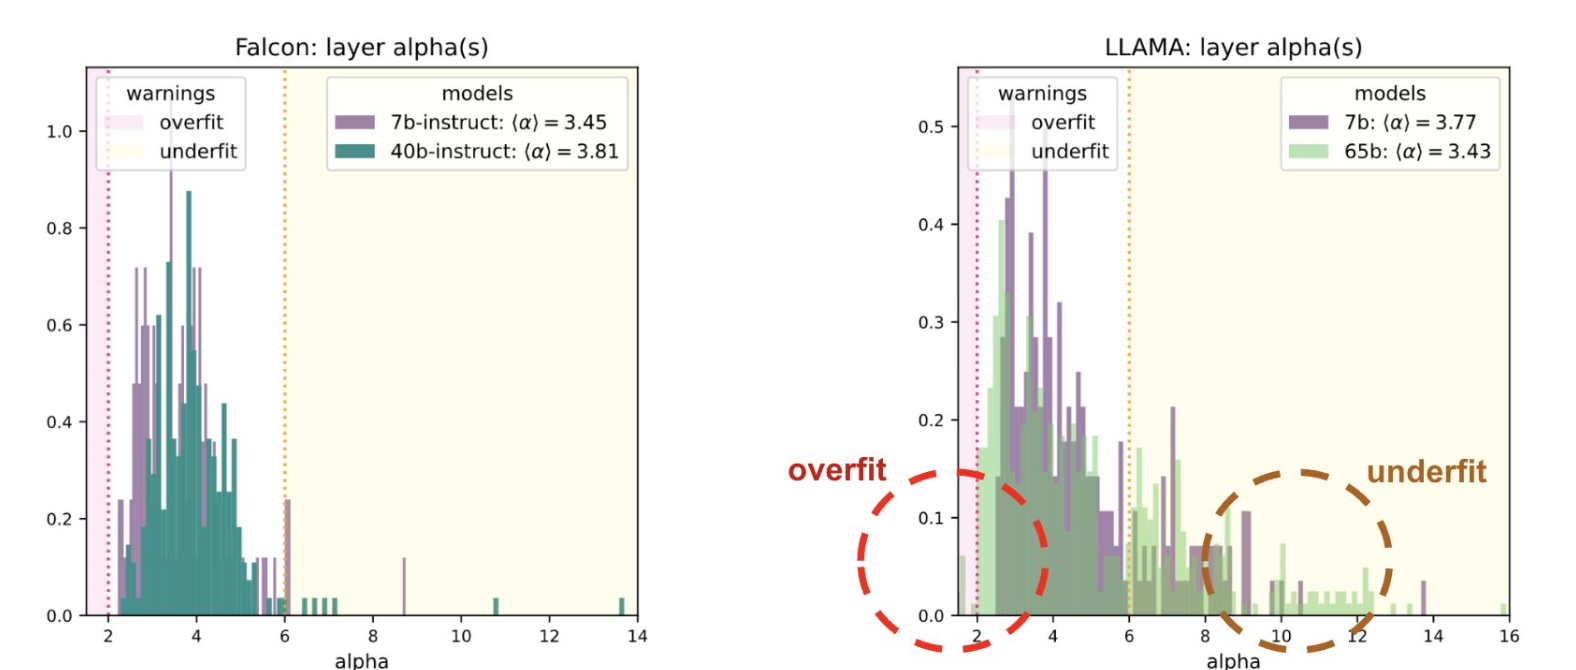
\includegraphics[width=15cm]{./img/falcon_vs_llama.png}
    \caption{Falcon vs Llama}
   \label{fig:falcon_vs_llama}
\end{figure}

For the Falcon-40b model, all of the layer \ALPHA range between $\alpha\in[2,6]$,
and therefore lie in the Fat-Tailed Universality class (in Table~\ref{tab:Uclass})
and are well-fit.
In contrast, looking at the Llama-40b layer \ALPHA, very many have $\alpha>6$,
indicating these layers are under-fit, and while a few have $\alpha <2$, suggesting
these are over-fit.  Finally, there are more layers with $\alpha~\sim2$ in Llama-65
vs Falcon-40b.

The observations on Llama-2 suggest that the layers with $\alpha\le 2$
are compensating for the layers with $\alpha>6$, and yielding suboptimal
performance for the Llama-65b architecture.
Based on these observations, we hypothesize that, in a multi-layer-perceptron (MLP),
when one layer does not or can not learn, then other layers will
have to compensate, and will be overloaded with the training data,
leading to $\alpha<2$, and even the \TRACELOG condition $\Delta \lambda_{min} < 0$.

%In Section~\ref{sxn:empirical} below, we will test this hypothesis in a 3-layer MLP model
%(MLP3), trained on MNIST, but only training 1 (FC1 or FC2), while keeping the other 2 frozen.
%In this way, we can simulate the situation seen above in the Llama-65b model,
%and observe the formation of a VHT ESD in the layer being trained.

%Additionally, as argued below, we conjecture that when $\alpha<2$, the model
%enters a kind-of glassy meta-stable phase, similar to the kinds of phases
%predicted by classic \STATMECH theories of learning.  A
%\nred{explain idea that VHT is \ATypical}

%We will explore how far we can push this analogy in our experiments to stress test the \SETOL approach.
%In particular, we will see effects reminiscent of a glassy system-the slowing down
%of the dynamics (in Sections~\ref{sxn:fc1})
%and a kind of hysteresis (Section~\ref{sxn:hysteresis_effect})

In Section~\ref{sxn:hysteresis_effect}, we will test this hypothesis.
By reducing the trainable parameters in a small MLP, we can simulate the situation seen above in the Llama-65b model,
and observe the formation of a Very Heavy Tailed (VHT) ESD in the dominating layer weight matrix.
Overloading results from having too few parameters for the complexity of the task. Adding more data increases 
the load up to the total complexity of the task itself.
%\st{Adding noisy labels increases the load up to the capacity of the a}

Moreover, we will also argue that in our experiments,
the model enters a kind of glassy meta-stable  phase, similar to the kinds of phases predicted by
classic \STATMECH theories of learning~\cite{SST92}
(described below).
Section~\ref{sxn:hysteresis_effect} will explore how far we can push the analogy of glassy systems in our experiments to 
stress test the \SETOL approach. In particular, we will see effects such as the slowing down of its dynamics, leading to a kind 
of hysteresis, specific to the under-parameterized regime.






